\documentclass[conference]{IEEEtran}
\IEEEoverridecommandlockouts
\usepackage{cite}
\usepackage[strings]{underscore}
\usepackage{stfloats}
\usepackage{amsmath,amssymb,amsfonts}
\usepackage{algorithm}
\usepackage{algorithmic}
\usepackage{graphicx}
\usepackage{textcomp}
\usepackage{xcolor}
\def\BibTeX{{\rm B\kern-.05em{\sc i\kern-.025em b}\kern-.08em
    T\kern-.1667em\lower.7ex\hbox{E}\kern-.125emX}}
\begin{document}

\title{Bisers: An Efficient DHCPv6 Bounding Solution}

\author{
  \IEEEauthorblockN{1\textsuperscript{st} Quan Zhang}
  \IEEEauthorblockA{\textit{School of Cyber Science and Engineering} \\
    \textit{Zhengzhou University}\\
    Zhengzhou, China \\
    vhqr@gs.zzu.edu.cn}
  \and
  \IEEEauthorblockN{2\textsuperscript{nd} Yi Guo \thanks{* Yi Guo is corresponding author.}}
  \IEEEauthorblockA{\textit{Information Engineering University} \\
    Zhengzhou, China \\
    nongfu16@hotmail.com}
  \and
  \IEEEauthorblockN{3\textsuperscript{rd} Baolei Mao}
  \IEEEauthorblockA{\textit{School of Cyber Science and Engineering} \\
    \textit{Zhengzhou University}\\
    Zhengzhou, China \\
    baoleimao@zzu.edu.cn}
  \and
  \IEEEauthorblockN{4\textsuperscript{th} Liancheng Zhang}
  \IEEEauthorblockA{\textit{Information Engineering University} \\
    Zhengzhou, China \\
    liancheng17@aliyun.com}
}

\maketitle

\begin{abstract}
  Network scanning is essential to penetration testing, but the IPv6
  network is difficult to scan because of the ample address space. For
  IPv6 networks managed using DHCPv6, detecting a precise range of
  DHCPv6 server assigned addresses helps narrow the scope of network
  scanning. For a DHCPv6 server that uses a continuous address
  allocation strategy, the boundary of this range is the first and
  last address it allocates; For a DHCPv6 server that uses a random
  address allocation strategy, this range is its address pool. We call
  the process of finding this range the DHCPv6 bounding. In this
  paper, we propose Bisers, an efficient DHCPv6 bounding solution that
  can quickly and accurately implement DHCPv6 bounding and effectively
  help scan IPv6 networks managed using DHCPv6.
\end{abstract}

\begin{IEEEkeywords}
  IPv6, DHCPv6, Network Scanning
\end{IEEEkeywords}

\section{Introduction}

Network scanning is an essential part of penetration testing. The
limited address space of IPv4, just 32 bits, makes it impossible for
an IPv4 network to withstand an attacker's scanning of the network:
Stateless scanning tools like Zmap scan the entire IPv4 network in a
matter of hours \cite{adrian_zippier_nodate}, and it usually takes
only a few minutes to scan a subnet. IPv6 extends the address space of
IPv4 to 128 bits, and the larger address space makes it difficult to
implement traditional network scanning methods. Therefore, finding a
new way to scan the IPv6 network is necessary.

IPv6 addresses are configured in two ways, SLAAC (Stateless Address
Automation) and DHCPv6 (Dynamic Host Configuration Protocol Version
6). SLAAC automatically generates addresses based on the network
prefix of the router advertised. While it is convenient enough to
configure the network, it is not easy to track the status of the IPv6
network. For example, look for nodes that use an IPv6 address at some
point. As a result, SLAAC cannot meet requirements such as network
traceability. Compared to SLAAC, DHCPv6 is widely used for client
tracking support and rich network parameter configuration.

For IPv6 networks managed using DHCPv6, detecting the range of DHCPv6
server assigned addresses helps narrow the scope of network
scanning. For a DHCPv6 server that uses a continuous address
allocation strategy, the boundary of this range is the first and last
address it allocates; For a DHCPv6 server that uses a random address
allocation strategy, this range is its address pool. We call the
search for this range DHCPv6 bounding.

Bergenholtz et al. \cite{bergenholtz_finding_2019} proposed DeHCP
(Algorithm \ref{algoDeHCP}), a bounding algorithm for DHCPv6 servers
using a continuous address allocation strategy. The DeHCP algorithm
uses a binary search method to search the range's boundary and avoids
errors by adding windows to complete the bounding quickly and
accurately.

\begin{algorithm}[H]
  \caption{DeHCP}
  \label{algoDeHCP}
  \renewcommand{\algorithmicrequire}{\textbf{Input:}}
  \renewcommand{\algorithmicensure}{\textbf{Output:}}
  \begin{algorithmic}[1]
    \REQUIRE Search range [a, b], Window size w
    \ENSURE Lower boundary lb
    \STATE host $\gets$ (a + b) / 2
    \STATE if a $\ge$ b then return host
    \STATE if Ping(host) then return DeHCP(a, host-1, w)
    \STATE for h in host-w ... host+w:
    \STATE \ \ if Ping(h) then return DeHCP(a, h-1, w)
    \STATE return DeHCP(host+1, b, w)
  \end{algorithmic}
\end{algorithm}

However, DeHCP only targets DHCPv6 servers that use a continuous
address allocation strategy. To compensate for the shortcoming of
DeHCP, we propose two bounding algorithms for DHCPv6 servers using a
random address allocation strategy: RDeHCP and SDeHCP. The former is
based on a detail of DHCPv6 implementation, which can be precisely
bounding. The latter estimates the boundary of the address pool based
on mathematical statistics, which is not as accurate as the former but
is generally effective. Combining these three algorithms, we propose a
perfect DHCPv6 bounding solution: Bisers (Binary Search \& Rebound \&
Solicit), which selects different bounding algorithms for servers with
different features. Fig~\ref{figBisers} shows the process of the
Bisers, divided into three phases: server discovery, server feature
detection, and bounding. We will describe the Bisers in more detail
later.

\begin{figure}[tbp]
  \centerline{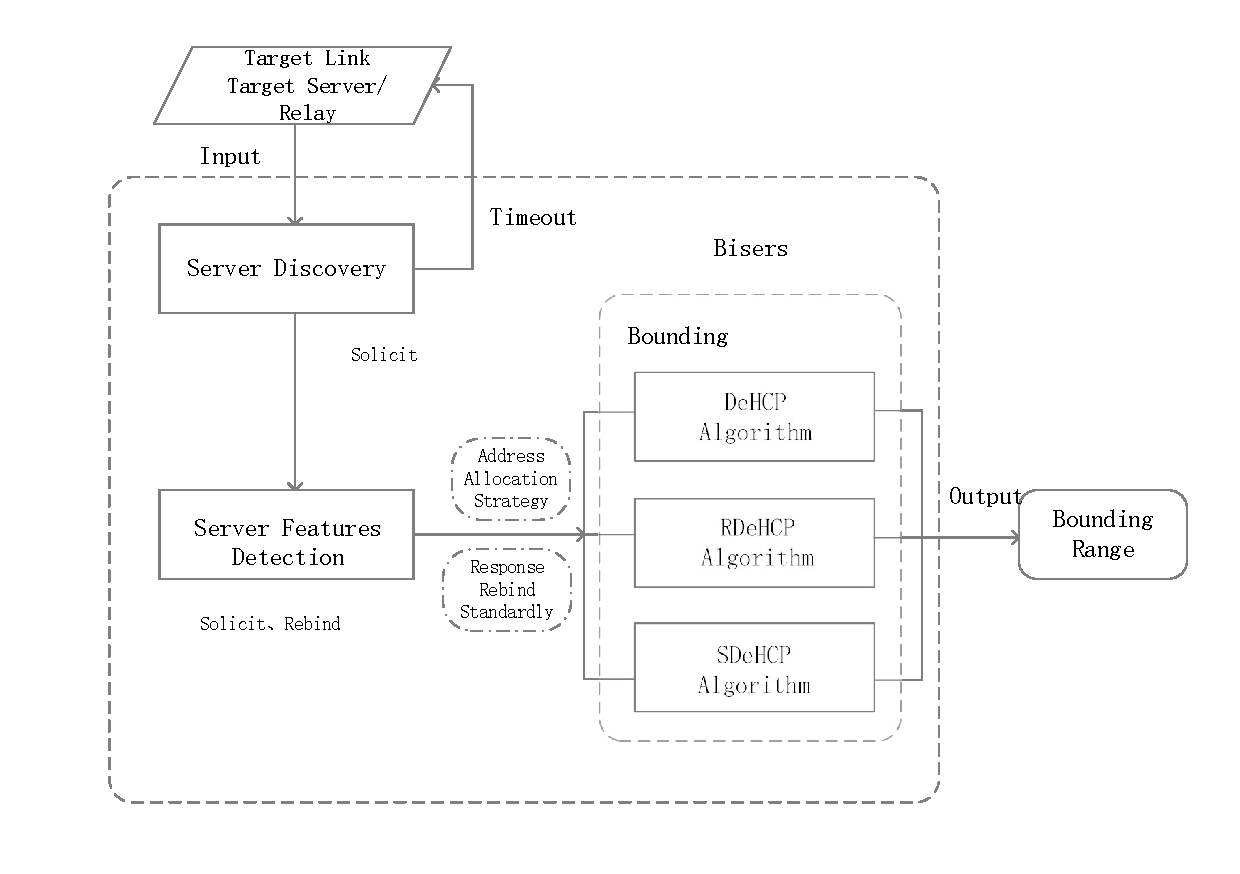
\includegraphics[scale=0.4]{bisers.pdf}}
  \caption{Bisers}
  \label{figBisers}
\end{figure}

We introduced Bisers' reference implementation on Linux:
https://github.com/vhqr0/bisers.

\section{DHCPv6 Protocol and Address Allocation Strategy Analysis}

The DHCPv6 client communicates with the server through
multicast-unicast, using the DUID specified server when
necessary. DHCPv6 centralizes the management of multiple links to a
single server through a relay mechanism \cite{carney_dynamic_2003}
\cite{mrugalski_dynamic_2018}, with one relay at each link. These
relays behave like servers, but instead of processing requests
directly, they encapsulate the request as a relay message agent to the
server or higher. Relay messages contain a link address field from
which the server judges the client's link and
responds. Fig~\ref{figRelay} shows the client requesting an address
from the server through two different modes of communication.

\begin{figure}[tbp]
  \centerline{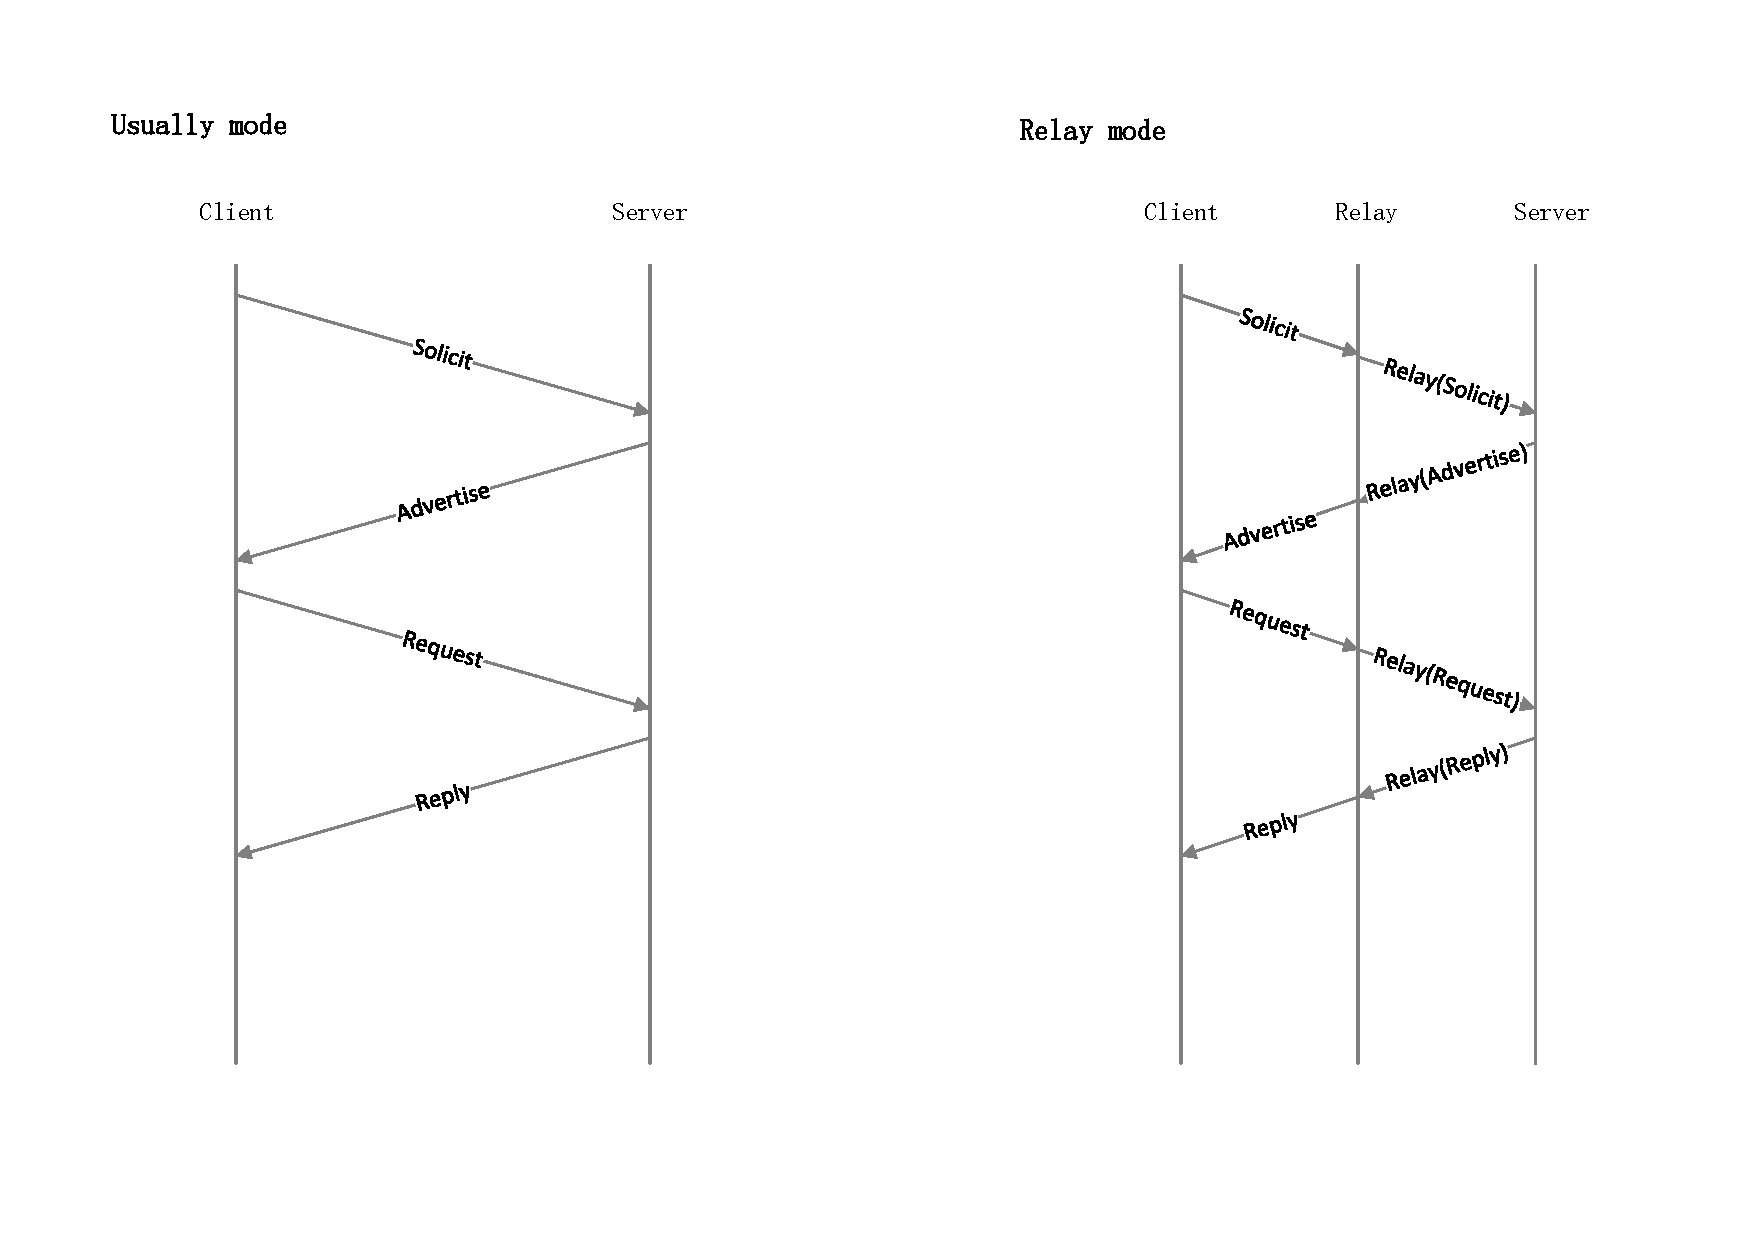
\includegraphics[scale=0.3]{relay.pdf}}
  \caption{Two modes of communication}
  \label{figRelay}
\end{figure}

The client discovers the server through the Solicit-Advertise process,
selects one of the discovered servers as the default server, and
requests an address from the server through the Request-Reply
process. Each address allocated by the server contains the values T1
and T2, representing renewal and rebinding timeouts, respectively. The
client should renew the address through the Renew-Reply process within
T1 time or rebind the address through the Rebind-Reply process after
T2 time.

The DHCPv6 specification does not specify how the server should
allocate an address. Early implementation of DHCPv6 followed DHCP's
continuous address allocation strategy, but it soon became apparent
that this allocation strategy had severe privacy issues. Therefore,
modern, security-oriented DHCPv6 implementations use random address
allocation strategies.

\section{DHCPv6 Bounding Solution Based on Multi-Type Message Detection}

The basic idea of the Bisers is to detect the features of the target
server with a small number of DHCPv6 requests and select an
appropriate bounding algorithm. Bisers are divided into three phases:
server discovery, server feature detection, and bounding. During the
server discovery phase, find and determine how to access the target
server. During the server feature detection phase, the critical
features of the target server are detected by a small number of
requests, and the corresponding bounding algorithm is selected. During
the bounding phase, the selected bounding algorithm is executed. We
will describe these three phases in more detail later.

\subsection{DHCPv6 Server Discovery}

Bisers determine how to access the target DHCPv6 server based on the
user's local and target links. If the target link is local, the local
server or relay can be accessed in the usual way. Otherwise, the
target server needs to be accessed by the relay, and the user needs to
provide the target link and the target server or relay.

Fig~\ref{figRelay2} shows how to access the target server through a
relay: the attacker mimics a DHCPv6 relay that encapsulates the
request in a relay message to the target server or an accessible
relay, with the link address field of the relay message as the target
link. The request is then surrogate to the target server, which
response based on the link address field and eventually returns the
response to the attacker similarly.

\begin{figure}[tbp]
  \centerline{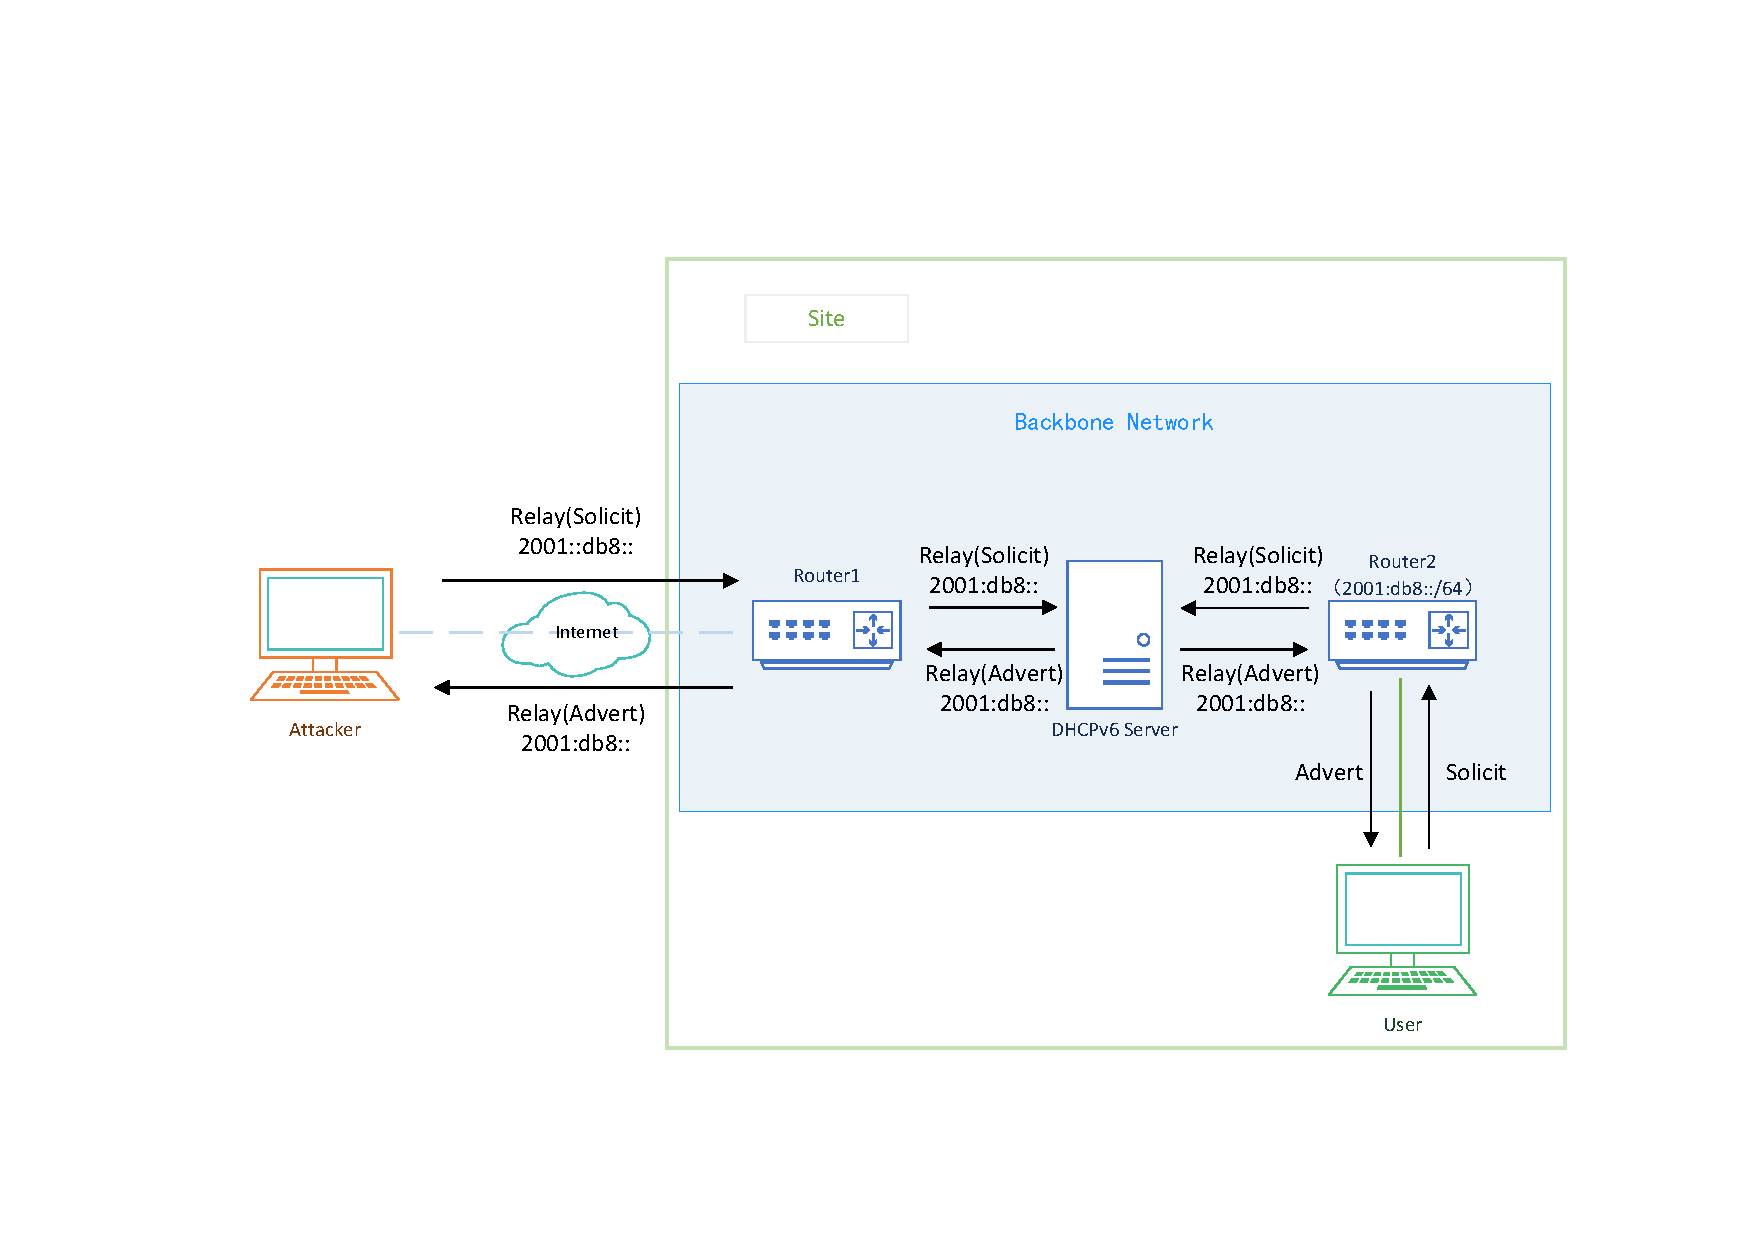
\includegraphics[scale=0.33]{relay2.pdf}}
  \caption{Illegal access to DHCPv6 Server}
  \label{figRelay2}
\end{figure}

Suppose the user's local and target links are on the same site. In
that case, the local link relay or server can be used
directly. Otherwise, users can look for target link routers through
tools such as traceroute, which typically relay for sites centrally
managed using DHCPv6 relays.

Once access is determined, the accessibility of the target server is
checked through a Solicit. The user must continue looking for the
server or relay if a timeout occurs.

\subsection{DHCPv6 Server Feature Detection}

To select a bounding algorithm that works for the target server,
Bisers needs to know two features of the target server: the address
allocation strategy and how the target server handles Rebind requests.

Bisers determine the address allocation strategy for the target server
by requesting two addresses and determining whether they are
continuous. If the two addresses are continuous, the allocation
strategy is continuous, and the DeHCP algorithm is selected.

If the target server uses a random address allocation strategy, the
way, the target server handles Rebind requests continues to be
detected. Bisers rebinds the address before and after the address
requested in the server discovery phase. If one succeeds, consider
that the target server is processing the Rebind request following the
standard and select the RDeHCP algorithm, or else select the SDeHCP
algorithm.

In summary, we present an algorithmic description at this phase: first
request two addresses $a1, a2$, and if $|a1-a2| = 1$, select DeHCP,
otherwise Rebind $a1-1$ and $a1+1$, and if successful, select RDeHCP
or SDeHCP.

At this phase, we can also detect other features of the target server,
such as:

\begin{itemize}
\item DUID, which can track a device across the network
  \cite{tront_security_2011} \cite{noauthor_what_nodate}.
\item Support for Rapid Commit, which may be under DOS attack
  \cite{carney_dynamic_2003} \cite{mrugalski_dynamic_2018}.
\item Support for Lease Query, which may leak more information \cite{zeng_dhcpv6_2007}.
\end{itemize}

These additional information can be used as an extension of the
specific implementation of Bisers.

\subsection{DHCPv6 Bounding}

Bisers finish the bounding by implementing the algorithm selected in
the previous phase. Below are two bounding algorithms proposed for
DHCPv6 servers using a random address allocation strategy.

The RDeHCP algorithm is based on a detail of DHCPv6 implementation:
When a client Rebind addresses, the server should decide to agree
based on its address allocation policy. Assuming that the server
agrees to Rebind unassigned address, ideally, we can quickly determine
whether an address is in the address pool with two requests, Ping and
Rebind. However, we cannot avoid an allocated address that we cannot
detect. Therefore, we avoid these errors with a windowed binary search
method similar to DeHCP. Change Ping in DeHCP to PingOrRebind, and we
get RDeHCP (Algorithm \ref{algoRDeHCP}).

\begin{algorithm}[H]
  \caption{RDeHCP}
  \label{algoRDeHCP}
  \renewcommand{\algorithmicrequire}{\textbf{Input:}}
  \renewcommand{\algorithmicensure}{\textbf{Output:}}
  \begin{algorithmic}[1]
    \REQUIRE Search range [a, b], Window size w
    \ENSURE Lower boundary lb
    \STATE host $\gets$ (a + b) / 2
    \STATE if a $\ge$ b then return host
    \STATE if PingOrRebind(host) then return RDeHCP(a, host-1, w)
    \STATE for h in host-w ... host+w:
    \STATE \ \ if PingOrRebind(h) then return RDeHCP(a, h-1, w)
    \STATE return RDeHCP(host+1, b, w)
  \end{algorithmic}
\end{algorithm}

The prerequisite of RDeHCP is that the target server treats Rebind
requests as standard, but we found that many DHCPv6 implementations
reject or do not even respond to any Rebind requests. For these
implementations, we propose SDeHCP (Algorithm \ref{algoSDeHCP}):
suppose the server randomly assigns an address in its address pool,
and the client requests $n+1$ address with minimum and maximum values
of $a', b'$, respectively. Numerically, we can calculate the
expectations of the address pool $[a'-delta, b'+delta]$, where
$delta = (b'-a')/n$. We take this as a bounding result.

\begin{algorithm}[H]
  \caption{SDeHCP}
  \label{algoSDeHCP}
  \renewcommand{\algorithmicrequire}{\textbf{Input:}}
  \renewcommand{\algorithmicensure}{\textbf{Output:}}
  \begin{algorithmic}[1]
    \REQUIRE Solicit times n
    \ENSURE Pool boundary [a', b']
    \STATE host $\gets$ Solicit()
    \STATE minhost $\gets$ host, maxhost $\gets$ host
    \STATE dotimes n:
    \STATE \ \ host $\gets$ Solicit()
    \STATE \ \ minhost $\gets$ min(host, minhost)
    \STATE \ \ maxhost $\gets$ max(host, maxhost)
    \STATE delta $\gets$ (maxhost - minhost) / n
    \STATE return [minhost - delta, maxhost + delta]
  \end{algorithmic}
\end{algorithm}

\section{Experiments and Analysis}

We introduced accuracy as a measure of the effect of bounding:
Assuming that the actual range is $[a, b]$ and the bounding algorithm
gets a range of $[a, b]$, we define accuracy as
$1-\frac{|b'-b|+|a'-a|}{b-a}$. We believe that the bounding algorithm
is accurate when its accuracy exceeds $98\%$. We do the simulation and
the actual test. The simulation experiment aims to select suitable
parameters for the three bounding algorithms. After determining the
default parameters, we selected several mainstream DHCPv6
implementations for actual testing to validate Bisers.

In the simulation experiment, we simulated a natural network
environment: a DHCPv6 server with a continuous or random address
allocation strategy and an 48-bit address pool. 1000 DHCPv6 clients,
and then leave some of them undetectable at $70\%$, $50\%$, and $30\%$
offline ratios, respectively. Different algorithms and parameters are
used to bound in different environments. The accuracy of DeHCP under
different window sizes and offline ratios is shown in Table
\ref{tabDeHCP}. RDeHCP remains $100\%$ accurate in three offline
ratios at window size 0, so we do not present the results. SDeHCP is
independent of network size and offline ratios and only tests accuracy
at 32, 64, 128, and 256 requests, as shown in Table
\ref{tabSDeHCP}. With $98\%$ accuracy, we selected suitable parameters
for three algorithms: DeHCP window size 4, RDeHCP window size 0, and
SDeHCP request times 128.

\begin{table*}[htbp]
  \caption{DeHCP experiment result.}
  \begin{center}
    \centering
    \begin{tabular}{|c|c|c|c|}
      \hline
      \textbf{Windows Size} & \multicolumn{3}{|c|}{\textbf{Offline Ratio}} \\
      \cline{2-4}
                            & 30\% & 50\% & 70\% \\
      \hline
      1 & 99.8\% & 91.16\% & 53\% \\
      2 & 99.8\% & 93.96\% & 83.22\% \\
      3 & 99.8\% & 98.54\% & 94.86\% \\
      4 & 99.8\% & 99.7\% & 98.7\% \\
      \hline
    \end{tabular}
    \label{tabDeHCP}
  \end{center}
\end{table*}

\begin{table*}[htbp]
  \caption{SDeHCP experiment result.}
  \begin{center}
    \begin{tabular}{|c|c|c|c|c|}
      \hline
      \textbf{Request times} & 32 & 64 & 128 & 256 \\
      \hline
      \textbf{Accuracy} & 96.34\% & 97.93\% & 98.97\% & 99.49\% \\
      \hline
    \end{tabular}
    \label{tabSDeHCP}
  \end{center}
\end{table*}

We selected several mainstream DHCPv6 implementations for testing:
TP-Link routers (TL-XDR1860), Cisco routers (IOS 7200), Openwrt soft
routers (19.07), ISC DHCP Server (4.4.1), and Windows DHCP Server
(Windows Server 2016), covering home routers, commercial routers, soft
routers, and software implementations. We summarize the features of
each of these implementations before testing the accuracy of one of
the Bisers' implementations on these servers, such as whether to
support relay, address allocation strategy, how to handle Rebind
requests and default address pool size. We tried to use the default
parameters during testing when configuring the server. Manual
configuration of a 24-bit address pool if required. Request and
discard 1000 addresses before testing. Test results are shown in Table
\ref{tabDHCPv6Server}.

\begin{table*}[htbp]
  \caption{Mainstream DHCPv6 implementations test results.}
  \begin{center}
    \begin{tabular}{|c|c|c|c|c|c|}
      \hline
      & \multicolumn{5}{|c|}{\textbf{DHCPv6 Implementations}} \\
      \cline{2-6}
      & TP-Link & Cisco & Openwrt & Windows & ISC \\
      \hline
      \textbf{Relay Support} & No & Yes & Yes & Yes & Yes \\
      \textbf{Address Allocation Strategy} & Continuous & Random & Random & Random & Random \\
      \textbf{Response Rebind Standardly} & No & No & No & No & Yes \\
      \textbf{Default Pool Size} & N/A & N/A & 8 & 64 & N/A \\
      \textbf{Accuracy} & 100\% & 99.2\% & 96.9\% & 99.1\% & 100\% \\
      \hline
    \end{tabular}
    \label{tabDHCPv6Server}
  \end{center}
\end{table*}

Based on our results, we believe the Bisers solution is accurate for
these DHCPv6 implementations. TP-Link routers are significantly
different from other implementations: This implementation follows the
DHCP's continuous address allocation strategy and does not support
relay. Although cross-link access is impossible, the DeHCP algorithm
can be applied directly in this case. Other implementations support
relay and use random address allocation strategies, and Bisers's help
in scanning IPv6 networks managed by these implementations depends on
the address pool size. Openwrt routers, for example, have an 8-bit
address pool and can be easily scanned. Windows DHCP Server has a
64-bit address pool that is difficult to scan. Cisco routers and ISC
DHCP Servers require manual configuration of address pools, and the
ease of scanning depends on the configuration of the network
administrator.

\section{Security Advise}

To prevent detection attacks like Bisers, we recommend two things from
a network administrator's perspective:

\begin{itemize}
\item To restrict illegal access to the DHCPv6 server, administrators
  should set strict firewall policies to restrict external access to
  the DHCPv6 server. Internally, a link layer filtering mechanism
  similar to DHCPv6 Shield \cite{gont_dhcpv6-shield_2015} or DHCPv6
  Guard \cite{noauthor_guard_nodate}, should be used to inspect DHCPv6
  relay packets.
\item When configuring an address pool for a DHCPv6 server,
  administrators should configure an address pool that is too large to
  scan based on the address pool range known to the attacker.
\end{itemize}

\section{Conclusions}

The proposed Bisers solution can quickly and accurately complete
DHCPv6 bounding, with the advantages of remote detection, high speed,
and high accuracy, and can effectively help scan IPv6 networks managed
using DHCPv6.

\section*{Acknowledgment}

This work was supported by the National Natural Science Foundation of
China (Grant No. 62004176), the Key R\&D and promotion projects of
Henan Province (Grant No. 212102310989) and the Key Scientific
Research Projects of Higher Education Institutions in Henan Province
(Grant No. 21A520041).

\bibliographystyle{IEEEtran}
\bibliography{cites}

\end{document}